\chapter{Kiến trúc tổng thể}

\section{Nguyên tắc kiến trúc}

Bốn nguyên tắc chi phối mọi quyết định thiết kế trong hệ thống:

\begin{enumerate}[leftmargin=1.4em]
  \item \textbf{Không gọi chéo dịch vụ trực tiếp.} Ứng dụng và trang quản trị luôn đi
  qua gateway. Backend gọi AI service qua một \en{client} duy nhất
  (\code{app/clients/ai\_service\_client.py}); AI service gọi ngược backend qua một
  đường nội bộ duy nhất (\code{LEARNER\_STATE\_API\_URL}). Không có ngoại lệ nào khác.
  \item \textbf{Bất đồng bộ toàn phần ở tầng dịch vụ.} Mọi truy vấn cơ sở dữ liệu ở
  backend đều \code{async}/\code{await} với SQLAlchemy 2.0; không tồn tại phiên đồng bộ.
  \item \textbf{Một cửa vào cho mỗi động cơ mô hình hoá người học.} Trạng thái khái niệm
  chỉ được cập nhật qua \code{record\_concept\_observation}; điểm kỹ năng chỉ qua
  \code{record\_exercise\_results\_for\_user}. Trước đây có ba bản sao của chuỗi
  "nhận sự kiện $\rightarrow$ tra mã sự kiện $\rightarrow$ áp dụng", và chúng đã phân kỳ.
  \item \textbf{Kiến trúc sạch ở phía client.} Flutter tách \code{data/} $\rightarrow$
  \code{domain/} $\rightarrow$ \code{presentation/}; tầng \code{domain} không bao giờ
  phụ thuộc \code{presentation}.
\end{enumerate}

\section{Sơ đồ kiến trúc}

\begin{figure}[htbp]
\centering
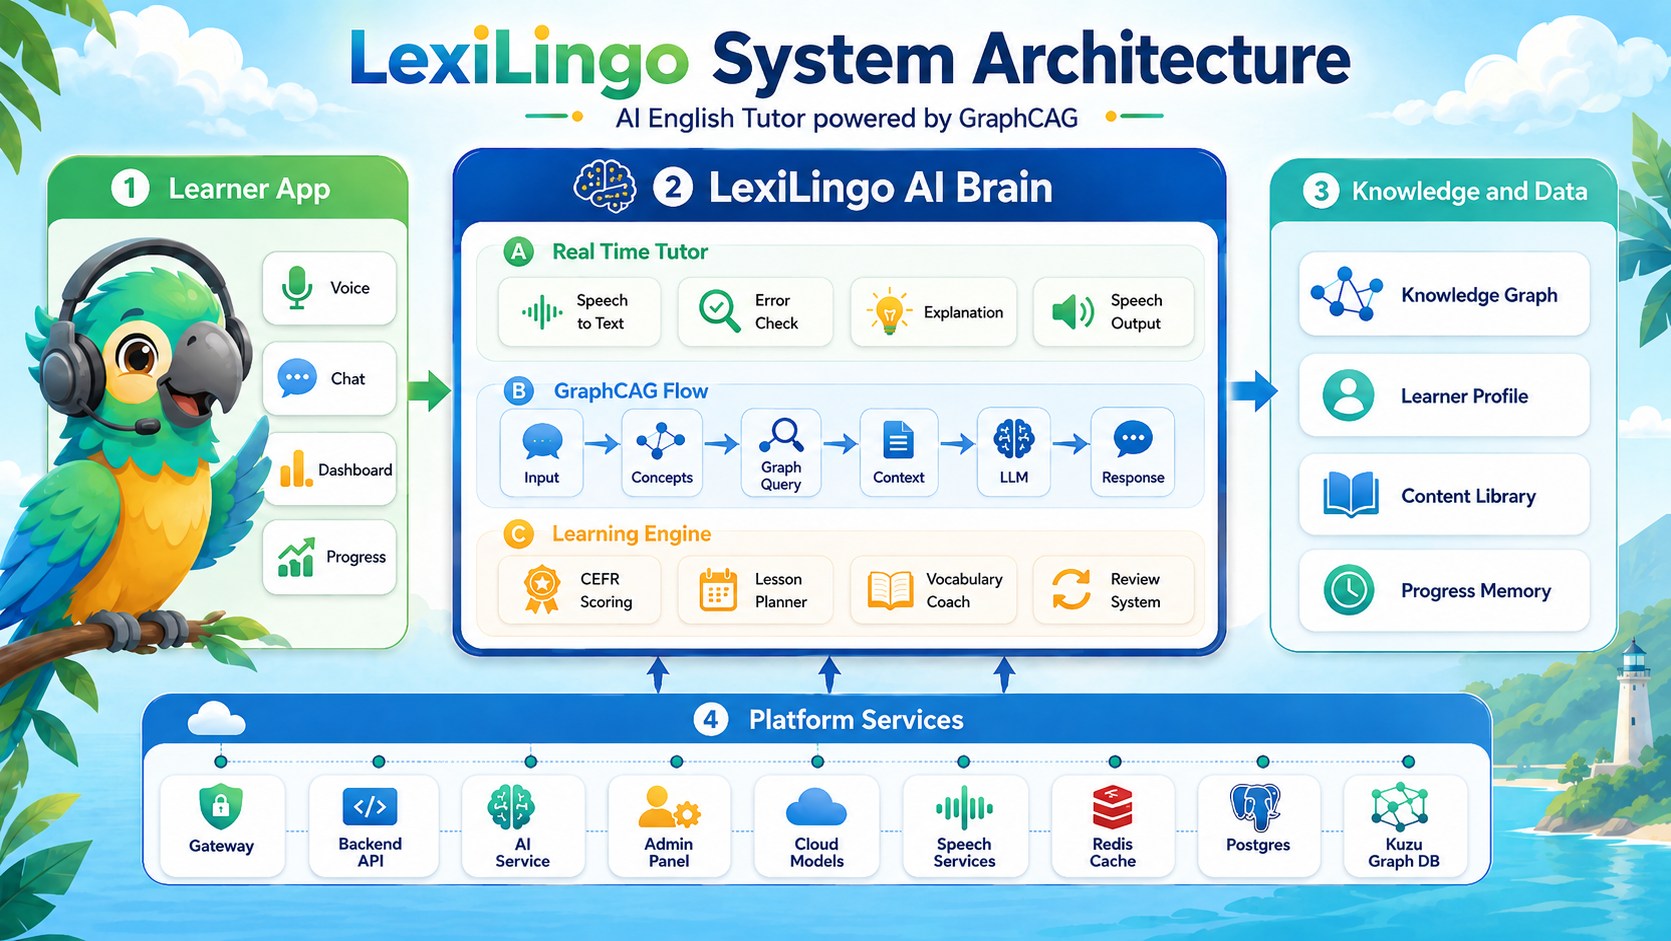
\includegraphics[width=\textwidth]{../architecture_lexilingo.png}
\caption{Kiến trúc tổng thể LexiLingo: tầng client, gateway, dịch vụ và dữ liệu}
\end{figure}

Mô tả theo tầng:

\begin{longtable}{L{2.8cm} L{11.0cm}}
\toprule
\textbf{Tầng} & \textbf{Thành phần và vai trò}\\
\midrule
\endhead
Client & Ứng dụng Flutter (người học), trang quản trị React (quản trị viên), MCP client (lập trình viên/tác tử AI trong IDE).\\
Gateway & Nginx 1.27-alpine: kết thúc TLS, định tuyến \code{/api/v1/*} về backend và \code{/ai/*} về AI service, giới hạn tần suất, chặn theo \en{WAF} biên (Cloudflare).\\
Dịch vụ & \code{backend-service} (cổng 8000) — nghiệp vụ; \code{ai-service} (cổng 8080) — AI; hai tiến trình phụ \code{backend-reminder-worker} và \code{backend-reminder-beat} chạy Celery.\\
Dữ liệu & PostgreSQL (nguồn sự thật nghiệp vụ), Redis (bộ nhớ đệm, phiên, hàng đợi Celery, bộ nhớ đệm đồ thị con), MongoDB (hội thoại, tạo tác AI, vùng đệm quan sát), KuzuDB (đồ thị tri thức nhúng).\\
Quan trắc & Prometheus thu thập chỉ số, Grafana hiển thị; nhật ký có \code{X-Request-ID} xuyên suốt.\\
\bottomrule
\caption{Các tầng trong kiến trúc}
\end{longtable}

\section{Luồng một yêu cầu điển hình}

Ví dụ: người học hoàn thành một bài học.

\begin{enumerate}[leftmargin=1.4em]
  \item Flutter gọi \code{POST /api/v1/learning/lessons/\{id\}/complete} kèm
  \en{JWT} (\en{JSON Web Token} — thẻ xác thực có chữ ký) trong tiêu đề \code{Authorization}.
  \item Nginx kiểm tra tần suất, gắn \code{X-Request-ID}, chuyển tiếp về backend.
  \item Backend chạy chuỗi \en{middleware}: kiểm tra máy chủ tin cậy $\rightarrow$ CORS
  $\rightarrow$ giới hạn tần suất $\rightarrow$ sinh mã yêu cầu $\rightarrow$ ghi nhật ký.
  \item Bộ định tuyến giải mã JWT, nạp người dùng, kiểm tra quyền.
  \item Tầng dịch vụ ghi \code{LessonCompletion}, cộng XP (\code{xp\_service}), cập nhật
  chuỗi ngày học (\code{streak\_service}), kiểm tra thành tích
  (\code{achievement\_checker\_service}).
  \item Kết quả từng bài tập được đẩy vào \code{record\_exercise\_results\_for\_user}:
  cập nhật \code{UserSkillScore} (điểm kỹ năng CEFR) và, nếu bài tập có
  \code{concept\_id}, gọi tiếp \code{record\_concept\_observation} để lập lịch ôn tập FSRS.
  \item Phản hồi trả về client; các tác vụ chậm (thông báo đẩy, tổng hợp thống kê) được
  đưa sang Celery.
\end{enumerate}

\begin{luuy}[Vì sao tách hai động cơ]
Điểm kỹ năng trả lời câu hỏi \textit{"người học đang ở bậc CEFR nào?"}; trạng thái khái
niệm trả lời \textit{"khi nào cần ôn lại khái niệm này?"}. Hai câu hỏi này có chu kỳ cập
nhật và ngữ nghĩa khác nhau, nên gộp chung sẽ làm hỏng cả hai. Điều bắt buộc là mọi hoạt
động có chấm điểm phải đến được cả hai động cơ.
\end{luuy}

\section{Ranh giới trách nhiệm giữa backend và AI service}

Đây là ranh giới hay bị hiểu nhầm nhất, nên được nêu rõ:

\begin{longtable}{L{6.8cm} L{6.8cm}}
\toprule
\textbf{backend-service} & \textbf{ai-service}\\
\midrule
\endhead
Nguồn sự thật về người học: tài khoản, tiến độ, XP, từ vựng, khoá học, trạng thái khái niệm. &
Không sở hữu dữ liệu người học; đọc/ghi qua API nội bộ của backend.\\
PostgreSQL là kho chính. & MongoDB (hội thoại, tạo tác), KuzuDB (đồ thị tri thức dùng chung), Redis (đệm).\\
Quyết định thăng bậc CEFR, mở khoá nội dung, trao thưởng. & Quyết định nội dung phản hồi, chiến lược sư phạm, chẩn đoán lỗi.\\
Mất dịch vụ $\Rightarrow$ mất khoá học, đăng nhập, tiến độ. & Mất dịch vụ $\Rightarrow$ mất chat/dịch/giọng nói, \textbf{không} mất tiến độ.\\
Thời gian dựng lại ảnh Docker: khoảng 1 phút. & Khoảng 15--30 phút (bánh xe \code{llama-cpp-python}).\\
\bottomrule
\caption{Ranh giới trách nhiệm giữa hai dịch vụ lõi}
\end{longtable}

\section{Hợp đồng dữ liệu dùng chung}

Thư mục \code{contracts/} chứa các định nghĩa dữ liệu mà nhiều dịch vụ cùng dựa vào.
Trường hợp điển hình là \textbf{danh sách khoá được phép} (\en{allowlist}) của tải trọng
quan sát người học: nó được khai báo hai nơi — \code{app/schemas/learner\_state.py} phía
backend và \code{api/services/learner\_observation\_spool.py} phía AI service. Một khoá lạ
sẽ làm cả lô quan sát bị từ chối, nên khi thêm trường mới phải sửa đồng thời cả hai; bộ
kiểm thử \code{test\_content\_contract\_parity.py} tồn tại để chặn việc quên.
